\section{Fibrations and cofibrations}
\subsection{Comparing fibers over different points}
Let $p:E\to B$ be a fibration.
Above, we saw that this implies that paths in $B$ ``lift'' to paths in $E$.
Let us consider a path $\omega:I\to B$ with $\omega(0) = a$ and $\omega(1) = b$.
Denote by $F_a$ the fiber over $a$. If $p$ is a covering space, then 
unique path lifting provides us with a homeomorphism $F_a\to F_b$ depending
only on the homotopy class of the path $\omega$. Our first goal today is
to construct an analogous map for a general fibration. 

Consider the solid arrow diagram:
\begin{equation*}
    \xymatrix{
	F_a\ar[d]_{\mathrm{in}_0}\ar[rr] & & E\ar[d]^p\\
	I\times F_a\ar@{-->}[urr]^{h}\ar[r]^{\mathrm{pr}_1} & I\ar[r]^{\omega} & B.
    }
\end{equation*}
This commutes since $\omega(0) = a$.
Utilizing the homotopy lifting property, there is a dotted arrow that makes the entire diagram commute.
If $x\in F_a$, the image $h(1,x)$ is in $F_b$.
This supplies us with a map $f:F_a\to F_b$, given by $f(x) = h(1,x)$.

Since we are not working with a covering space, there will in general be
many lifts $h$ and so many choices of $f$. We may at least hope that the 
homotopy class of $f$ is determined by the homotopy class of $\omega$. 

So suppose we have two paths $\omega_0,\omega_1$, with $\omega_0(0) = \omega_1(0) = a$, and a homotopy $g:I\times I\to B$ between them (so that $g(0,t)=\omega_0(t)$, $g(1,t)=\omega_1(t)$, $g(s,0)=a$, $g(s,1)=b$). 
Choose lifts $h_0$ and $h_1$ as above. 
These data are captured by a diagram of the form
\begin{equation*}
    \xymatrix{
	((\partial I\times I)\cup (I\times \{0\}))\times F_a\ar[d]_{\mathrm{in}_0}\ar[rr] & & E\ar[d]^p\\
	I\times I\times F_a\ar[r]_{\mathrm{pr}_1}\ar@{-->}[urr] & I\times I\ar[r]_g & B
    }
\end{equation*}
The map along the top is given by $h_0$ and $h_1$ on 
$\partial I\times I\times F_a$ and by $pr_2:I\times F_a\to F_a$ followed by
the inclusion on the other summand. 

The dotted lift would restrict on $I\times\{1\}\times F_a$ 
to a homotopy between $f_0$ and $f_1$. 

% Add a picture, maybe?
%
%Think of the space $(\partial I\times I)\cup (I\times 0)$ as follows:
%\begin{equation*}
%\begin{tikzpicture}
%    \draw (2,2) -- (0,2) -- (0,0) -- (2,0);
%    \node [above] at (1,2) {$h_1$};
%    \node [below] at (1,0) {$h_0$};
%    \node [left] at (0,1) {$in_0$};
%\end{tikzpicture}
%\end{equation*}
%and $I\times I$ looks like:
%\begin{equation*}
%    \begin{tikzpicture}
%	\draw (0,0) -- (0,2) -- (2,2) -- (2,0) -- (0,0);
%	\draw[fill] (2,2) circle [radius=0.05];
%	\draw[fill] (2,0) circle [radius=0.05];
%	\node [left] at (0,1) {$a$};
%	\node [above] at (1,2) {$\omega_1$};
%	\node [below] at (1,0) {$\omega_0$};
%	\node [right] at (2,1) {$b$};
%	\node [above right] at (2,2) {$f_1$};
%	\node [below right] at (2,0) {$f_0$};
%    \end{tikzpicture}
%\end{equation*}
%
%Does the dotted map exist? Clearly this is crying out for us to use the homotopy lifting property. But what should our space $W$ be? Well the following pair:
%\begin{equation*}
%    \begin{tikzpicture}
%	\draw (2,2) -- (0,2) -- (0,0) -- (2,0);
%    \end{tikzpicture}\subseteq
%    \begin{tikzpicture}
%	\draw (0,0) -- (0,2) -- (2,2) -- (2,0) -- (0,0);
%    \end{tikzpicture}
%\end{equation*}
%is homotopy equivalent to $(0\subseteq I)\times I$. Hence in our diagram we now have:

Well, the subspace $(\partial I\times I)\cup(I\times\{0\})$ of $I\times I$
wraps around three edges of the square. It's easy enough to create a 
homeomorphism with the pair $(I\times I,\{0\}\times I)$, so the HLP (with 
$W=I\times F_a$) gives us the dotted lift.

We will capture this fact in a statement about the action of paths. Recall that
the fundamental group of a pointed space $(X,*)$ acts on the fiber $p^{-1}(*)$
of any covering space $p:E\to X$. We have just shown that it also acts on the
homotopy type of the fiber of any fibration over $X$. It's useful to express
this in a way that does not specify a basepoint (and hence is meaningful
even for spaces that are not path connected). 
Recall that a {\em groupoid} is a small category in which every morphism
is an isomorphism.
\begin{definition}
    Let $X$ be a topological space.
    The \emph{fundamental groupoid} $\Pi_1(X)$ of $X$ is the groupoid
    whose objects are the points of $X$ and whose morphisms are the 
homotopy classes of paths in $X$.
    The composition of compatible paths $\sigma$ and $\omega$ is defined by:
    \begin{equation*}
	(\sigma\cdot\omega)(t) = \begin{cases}
	    \omega(2t) & 0\leq t\leq 1/2\\
	    \sigma(2t - 1) & 1/2\leq t\leq 1.
	\end{cases}
    \end{equation*}
\end{definition}
The results of the previous sections can be succinctly summarized as follows.
\begin{prop}
    A fibration $p:E\to B$ determines a functor $\Pi_1(B)\to\Ho\Top$.
\end{prop}
Note: Last semester we defined the product of loops as juxtaposition but in
the reverse order. That convention would have produced a contravariant functor
$\Pi_1(X)\to\Ho\Top$.

\subsection{Cofibrations}
Let $i:A\to X$ be a map of spaces.
If $Y$ is another space, when is the induced map $Y^X\to Y^A$ a fibration?
This is asking for the map $i$ to satisfy a condition ``dual'' to the 
fibration condition.

By the definition of a fibration, we want a lifting:
\begin{equation*}
    \xymatrix{
	W\ar[r]\ar[d]_{\mathrm{in}_0} & Y^X\ar[d]\\
	I\times W\ar@{-->}[ur]\ar[r] & Y^A\,.
    }
\end{equation*}
Adjointing over, we get:
\begin{equation*}
    \xymatrix{
	A\times W\ar[r]^{i\times 1}\ar[d]_{1\times \mathrm{in}_0} & X\times W\ar[d]\ar[ddr]& \\
	A\times W\times I \ar[r]\ar[drr] & X\times I\times W\ar@{-->}[dr] & \\
	& & Y\,.
    }
\end{equation*}
Adjointing over again, this diagram transforms to:
\begin{equation*}
    \xymatrix{
	A\ar[r]\ar[d] & X\ar[d]\ar[ddr] & \\
	A\times I\ar[r]\ar[drr] & X\times I\ar@{-->}[dr] & \\
	& & Y^W\,.
    }
\end{equation*}
This discussion motivates the following definition of a ``cofibration,''
dual to the notion of fibration.

\begin{definition}\label{cofibration}
A {\em cofibration} is a map $i:A\to X$ that satisfies 
    \emph{homotopy extension property} (sometimes abbreviated as ``HEP''):
    for any space $Y$, there is a dotted map in the following diagram that makes it commute:
    \begin{equation*}
    \xymatrix{
	A\ar[r]\ar[d] & X\ar[d]\ar[ddr] & \\
	A\times I\ar[r]\ar[drr] & X\times I\ar@{-->}[dr] & \\
	& & Y\,.
    }
    \end{equation*}
\end{definition}
By the universal property of a pushout, this is equivalent to the existence
of an extension in 
\begin{equation*}
    \xymatrix{
	X\cup_A (A\times I)\ar[r]\ar[dr] & X\times I\ar@{-->}[d]\\
	& Y\,.
    }
\end{equation*}
Now there is a univeral example, namely $Y=X\cup_A(A\times I)$. So a map
$i$ is a cofibration if and only if $X\cup_A (A\times I)$ is a retract of 
$X\times I$.

\begin{example}\label{intervalcofib}
    $S^{n-1}\hookrightarrow D^n$ is a cofibration.
    \todo{Properly draw out this figure!}
    \begin{figure}[H]
	\centering
	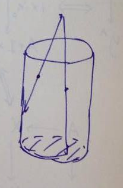
\includegraphics[scale=0.75]{retract-cofibration}
	\caption{Drawing by John Ni.}
    \end{figure}
    In particular, setting $n=1$ in this example, $\{0,1\}\hookrightarrow I$ is a cofibration.
\end{example}

The class of cofibrations is closed under the following operations.
\begin{itemize}
    \item Cobase change: if $A\to X$ is a cofibration and $A\to B$ is any map,
	the pushout $B\to X\cup_A B$ is again a cofibration.
    \item Coproducts.
    \item Composition.
\end{itemize}
Also, it satisfies the condition that we used to motivate the definition:
If $A\to X$ is a cofibration and $Y$ is an space, then $Y^X\to Y^A$ is a 
fibration. In particular, the map 
\[
ev_{0,1}:Y^I\to Y\times Y
\]
given by evaluation at the endpoints of the path is a fibration.

Finally, 
\begin{lemma} 
Any cofibration is a closed inclusion.
\end{lemma}

\begin{exercise}
An important (but easy!) fact about fibrations is that the canonical map 
$X\to \ast$ from any space $X$ is a fibration.
(Afficianados of model categories get excited about this 
because this says that all objects in the associated model structure on
topological spaces is fibrant.)
After all, this is a product projection! 
But the ``dual'' statement is false.    
Give an example of a compactly generated space $X$ containing a point
$*$ such that $\{*\}\hookrightarrow X$ is not a cofibration.
\end{exercise}
A basepoint $*$ is {\em nondegenerate} if $\{*\}\hookrightarrow X$ 
is a cofibration. 
If $\ast$ has a neighborhood in $X$ that contracts to $\{\ast\}$,
the inclusion $\ast\hookrightarrow X$ is a cofibration.
If $\ast$ is a nondegenerate basepoint of $A$, the evaluation map 
$\mathrm{ev}:X^A\to X$ is a fibration,
The fiber of $\mathrm{ev}$ over a basepoint of $X$ 
is exactly the space of pointed maps $X^A_*$.
